% \chapter{Validity of Transformers for Spectral Classification}
% \label{chap:chapter-3}
% \section{Creation of artificial spectra}
% \label{sec:creation}
% Creating large amounts of high signal-to-noise signals was essential to verifying 
% the application of a Vision Transformer. These signals needed to include the 
% basic features of supernova spectrum, such as the presence of a continuum, 
% absorption lines, and emission lines. The locations of these spectral features 
% in particular were not important, as long as each class of supernovae had consistent 
% features. The \texttt{GenData} class was created to generate these signals. 

% \subsection{Features of \texttt{GenData} class}
% \label{ssec:features}
% The \texttt{GenData} class must provide a means of generating a large number (order of $10^5$)
% of random spectra. These spectra must exhibit a consistent continuum, variable noise, 
% and a set of spectral features that are unique to arbitrary classes. In order to 
% accomplish this, the \texttt{GenData} class must first identify a domain in which 
% to place spectral features, noise, and the continuum. The continuum is a function across
% the domain that remains consistent for all samples, and examples can be found in Fig.~\ref{fig:continuumoptions}.
% A set number of spectral features are randomly placed within the domain. The number of spectral
% features is determined by the user. Then, each class (or type) of spectra is assigned 
% a random combination of these spectral features. This is to ensure that each class 
% has a unique set of spectral features, while maintaining a consistent location of features. 
% Once the different classes are specified, the creation of the spectra can begin.

% \begin{figure}
%     \centering
%     
\includegraphics[width=0.5\textwidth]{figures/blackbox.jpeg}
%     \caption{Examples of different continuum options
%     (from left to right: linear, linear increasing, linear decreasing, 
% exponential increasing, and exponential decreasing).}
%     \label{fig:continuumoptions}
% \end{figure}

% \subsection{Creation of spectra}
% \label{ssec:creation}
% Once the spectral features present in each class are determined, the spectra can 
% be constructed from the ground up. First, the continuum is created 

% The essential Some of the features of the \texttt{GenData} class are as follows:
% \begin{itemize}
%     \item The ability to generate a large number (order of $10^5$) of random spectra
%     \item The ability to generate spectra with a continuum
%     \item The ability to generate spectra with absorption lines
%     \item The ability to generate spectra with emission lines
%     \item The ability to generate spectra with a combination of all three
%     \item The ability to generate spectra with a combination of all three, but with 
%     different spectral features in each spectrum

% \end{itemize}
\chapter{Creation and Training of Spectral ViT}
\label{chap:methods}
% Methods to validate transformers (fake spectra), create training data (fake spectra), 
% train various models (V1.1, V1.2, V1.3, V2), to find optimal training for V2

In order to examine the effectiveness of the transformer architecture for supernovae
spectral classification, a series of steps were taken. First, an in-house transformer 
architecture was created based on the traditional ViT architecture \cite{dosovitskiy2020}, 
which was quickly found to be trainable on a synthetic dataset. Next, a synthetic dataset 
using DESI spectra was created under a variety of preprocessing conditions. The previously 
created CNN and new transformer architectures were trained on each variation of 
preprocessed data. Finally, these training sessions were then used to determine 
the optimal training conditions for non redshift corrected data. 
\section{Creation of Spectral ViT}\label{sec:SpecViT}
The Spectral ViT architecture was created to be a direct extension of the ViT architecture
\cite{dosovitskiy2020} to be used for spectral classification, coded in the \texttt{PyTorch}
deep learning framework. The Spectral ViT architecture is shown graphically in
Appendix~\ref{app:SpecViT}. The Spectral ViT architecture is
composed of three main components: the pre-processor, the encoder, and the classifier. 

The pre-processing component is responsible for taking the (already preprocessed)
input spectra and converting it into a series of vectors that the transformer can interpret. 
Considering a group of $N$ spectra, each with $10000$ pixels, the each group 
is split into a set number of patches (approximately 100). Each patch is then 
linearly mapped via a fully connected network to a vector three times the patch size.
The sample is now a set of of size $N\times101\times300$. 
A classification token of the sample dimensionality as the patches 
is then added to the beginning of each sample, initialized randomly. 
In order for the transformer to properly understand the positional relationship between each patch, an embedding 
is added to each patch. This embedding is a scalar function based on the size 
of the patch is calculated as follows: 
\begin{equation}
    \text{Embedding}_{ij} = \begin{cases} \sin\left(\frac{i}{10000^{(j / \text{patch size})}}\right) & \text{if } j \text{ is even} \\
    \cos\left(\frac{i}{10000^{((j - 1) / \text{patch size})}}\right) & \text{if } j \text{ is odd}\end{cases},
\end{equation}
where $i$ is the position of the patch in the vector, and $j$ is the position of the patch in the sample~\cite{vaswani2017}.
A visual representation of the embeddings for the sample is shown in Fig.~\ref{fig:embedding}. Once the 
embeddings are added element-wise to the patches, the resulting tensor (of size $N\times101\times300$) is then passed through the encoder. 
\begin{figure}[H]
    \centering
    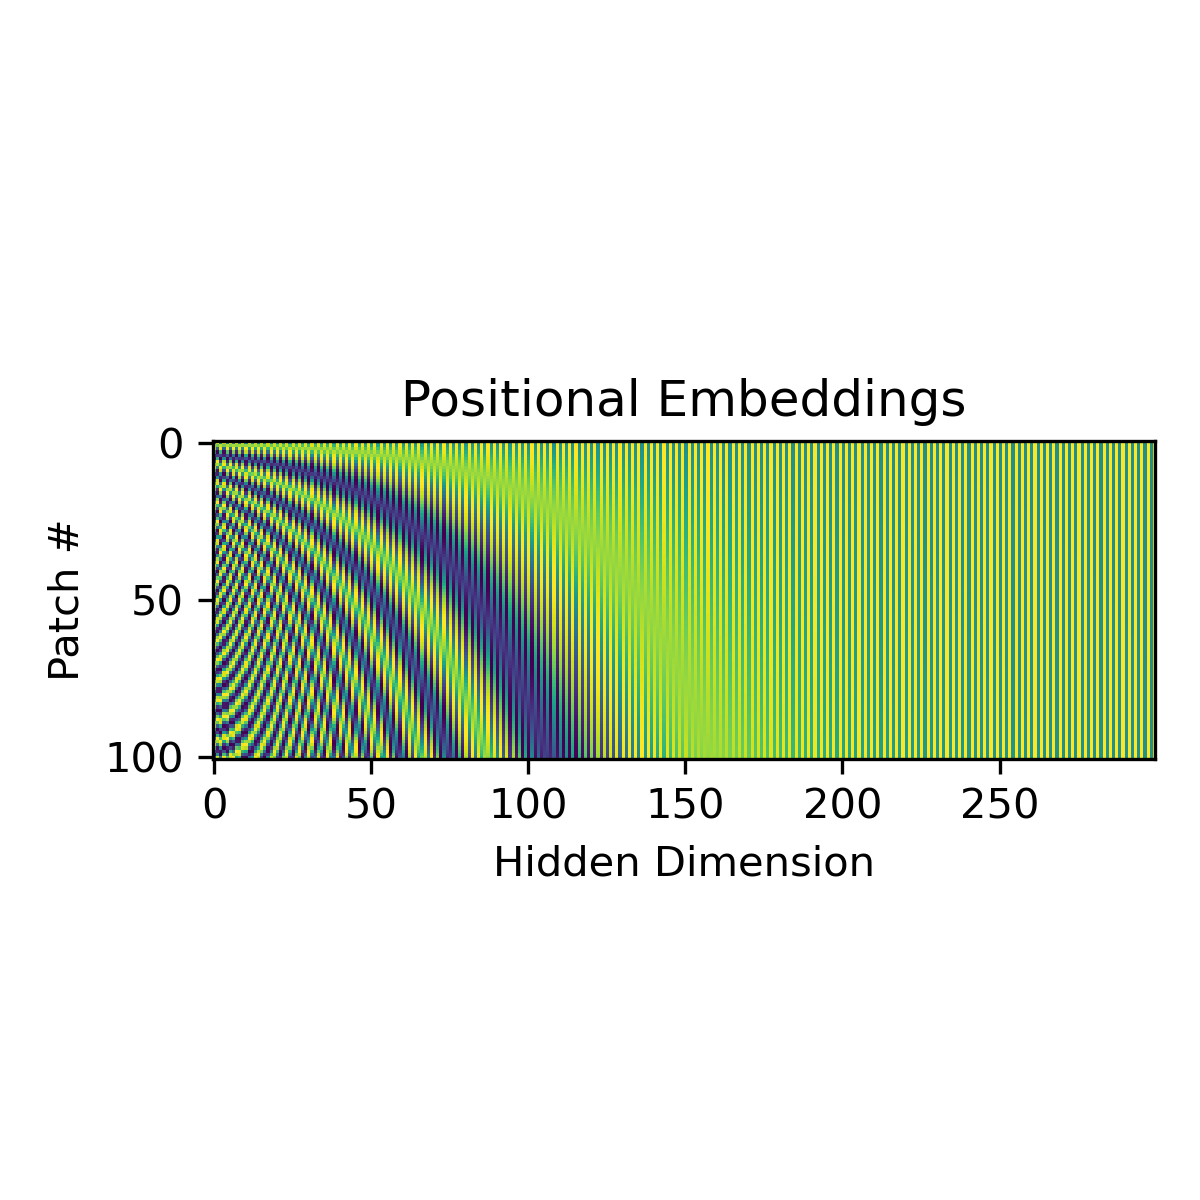
\includegraphics[width=.4\linewidth]{figures/embeddings.png}
    \caption{Visual representation of the embeddings for a sample of spectra split into 100 patches of length 300.}
    \label{fig:embedding}
\end{figure}

The encoder is the main component of any ViT architecture, as it contains the 
multi-head attention and feed-forward layers. The encoder is composed of a set number of
transformer blocks, each of which contains layer normalization, multi-head attention, another 
layer normalization, and finally a feed-forward layer. The multi-head attention layer 
is a scaled dot-product attention layer found in \textcite{vaswani2017}. Each patch 
is passed through three separate linear layers, each with a different set of weights, 
resulting in three sets of vectors: the query ($Q$), key ($K$), and value ($V$).
\begin{equation}
    \label{eq:mhsa}
    \text{Attention}(Q, K, V) = \text{softmax}\left(\frac{Q\cdot K^T}{\sqrt{d_k}}\right)\cdot V
\end{equation}
The dot-product between the query and key vectors is then calculated,
scaled by the square root of the dimensionality of the query vector, and then passed through a softmax function.
The resulting attention weights are then multiplied by the value vectors (Equation~\ref{eq:mhsa}). 
This is simultaneously done for each head in the multi-head attention layer. Each result is then 
concatenated together, and then passed through a linear layer to reduce the dimensionality
to the size of the query vector. This resulting vector is then added
element-wise to the original patches, normalized, and then passed through a MLP, 
resulting in a tensor of size $N \times 101 \times 300$. This again is added element-wise to the original patches. 
Each step is repeated for a set number of transformer blocks, resulting in a tensor of size
$N \times 101 \times 300$.

The final component of the Spectral ViT architecture is the classifier. The classifier
takes in only the first patch of each sample, which has been designated as the classification token.
The classification token is passed through a linear layer to reduce the dimensionality to the
number of classes, and then passed through a softmax function to produce a probability distribution
over the classes. Therefore, the resulting tensor is of size $N \times 1 \times 6$, for our 
6 classifications of supernovae.

\subsection{Validation of Spectral ViT Architecture}
\label{ssec:validation}
After the creation of the Spectral ViT architecture, ability to train effectively 
was tested. A synthetic dataset, consisting of a consistent continuum with 
Gaussian peaks placed at predetermined locations, was created. Certain combinations of 
peak locations were chosen to represent an arbitrary `class' of supernovae. These peaks, 
our synthetic emission lines, were given random amplitudes and widths, simulating  
variability, with a maximum allowed value. This maximum allowed value was then used to add 
Gaussian noise to the signal: either 2 or 5 times the signal to simulate noisy ($S/N=2$),
or very good data ($S/N=5$). Examples of the synthetic spectra with different continuum profiles 
are shown in Fig.~\ref{fig:synth_spectra}. 

These datasets with a signal-to-noise of 5 trivially separable by a smaller Spectral ViT architecture, 
which was able to achieve 100\% accuracy on the testing set. The lower quality data, however, 
was more difficult to separate, only achieving an 82\% test accuracy.

** PUT IN GRAPHS OF SYNTHETIC SPECTRA HERE **
** PUT IN GRAPHS OF TRAINING SYNTHETIC SPECTRA HERE **
** PUT IN TABLE OF TRAINING SYNTHETIC SPECTRA HERE - SN=2 and SN=5**

\section{Creation of Synthetic DESI Spectra}
\label{sec:synth_data}
Once the Spectral ViT architecture was shown to be able to train effectively on synthetic data,
the architecture was ready to be trained on DESI data. In order to create a large enough training 
set, authentic DESI spectra were used as a base to create synthetic spectra.

** Talk to BenZvi about what to put in this section / who to cite for all of the work **

\subsection{PreProcessing of DESI Spectra}
\label{ssec:preprocess}
% All of preprocessing including z correction and downsampling 
Once the spectra's were created and saved as DESI files, they needed to be 
extracted, preprocessed, split into training, testing, and validation sets, 
only then could they be saved, and used to train the Spectral ViT architecture.
The preprocessing method developed by ** Cite eddies paper **, and is split into 
3 main steps: z correction, rebinning / down sampling, and normalization. 

The Z correction step was used to move the spectra back into the rest frame using 
the redshift fitted to the original spectra by the DESI pipeline. Next, all artifacts 
in the spectra (masks, bad pixels, etc.) were removed. The spectra were then re-binned
and downsampled to a variable resolution (default 3600). Afterwards, the spectra were 
normalized by moving the max and min values to 1 and 0 respectively. Finally, for the 
CNN datasets, the spectra were split into a 2D array of equal height and width. 
After this, the spectra were split into training, testing and validation datasets that 
comprised of 60\%, 20\%, and 20\% of the total dataset, respectively.
\section{Training of Neural Networks}
\label{sec:training} 

\subsection{CNN Training}
\label{ssec:cnn_training}
CNN training was conducted using DESI spectra downsampled to a resolution of 3600, and 
put into a 2D array of equal height and width. The CNN architecture was developed 
by ** Cite eddies paper **, and has properties shown in Table~\ref{tab:cnn_architecture}.
This CNN was trained for a maximum of 50 epochs, with a batch size of 50, and 
non-variable hyperparameters (Table~\ref{tab:cnn_hyperparameters}). 
The timeline of the training of the CNN architecture is shown in Fig.~\ref{fig:cnn_training}.


\subsection{Transformer Training}
\label{sec:transformer_training}
The Spectral ViT architecture, idealistically, should have the capability to be trained 
on non rest-frame corrected spectra. In an effort to test how down-sampling had 
affected the training of the Spectral ViT architecture, the Spectral ViT architecture
was trained on various downsampling values. Based on these models, a downsampling 
value was chosen for non-rest-frame corrected spectra. The Spectral ViT architecture 
was trained on DESI spectra downsampled to a resolution of 3600, 1800, and 900. 
The Spectral ViT architecture was trained for a maximum of 100 epochs, with 
batch sizes of 50, and non-variable hyperparameters (Table~\ref{tab:transformer_hyperparameters}).
